\documentclass[a4paper,10pt,twoside]{article}

\usepackage[english]{babel}
\usepackage{amssymb}
\usepackage{fancyhdr}
\usepackage{graphicx}
\usepackage[ocgcolorlinks]{hyperref}
\usepackage{todonotes}
\usepackage{caption}
\usepackage{subcaption}

\pagestyle{fancy}
\fancyhead{}
\fancyfoot{}
\fancyhead[RE,LO]{de Kok \& Methenitis}
\fancyhead[RO,LE]{Week 3}
\fancyfoot[RE]{\thepage$\quad \square$}
\fancyfoot[LO]{$\square \quad$\thepage}

\title{Report for Week 3 \\\normalsize $k$-means \& Bag-of-Visual words\\ or how to create a Google Goggles-like system}

\author{Patrick de Kok (5640318) \and Georgios Methenitis (10407537)}

\begin{document}
\maketitle
\thispagestyle{empty}

\section{Individual steps of $k$-means}

\section{Running your implemented $k$-means}

\section{Color-based image segmentation}

\section{$k$-means, SIFT \& Bag-of-Words: calculating storage for raw SIFT}
Each SIFT vector has 128 elements.  Each element is represented by an integer\footnote{The binary invoked to extract the SIFT vectors returns integers.  However, the \texttt{read\_sift\_from\_file(sift\_path)} function interprets these as Python \texttt{float} objects.  In the standard Python implementation, CPython, a \texttt{float} always consists of 64 bits, which is 8 bytes.  This would result in quadrupling all final answers.}.  Assuming each integer consists of 2 bytes and there is no storage overhead for the vector, 1 SIFT vector needs 256 bytes of storage.  To store all 50,000 vectors that belong to one image, 12,800,000 bytes = $12.8 \cdot 10^6 B = 12.8 \mbox{ MB} \approx 12.21 \mbox{ MiB}$ is needed.  For Facebook's daily addition of new images, one needs $12.8 \cdot 10^6 \cdot 350 \cdot 10^6 \mbox{ B} = 4.48 \cdot 10^{15} \mbox{ B} = 4.48 \mbox{ PB} = 4,480,000,000 \mbox{ MB} = 4272460937.5 \mbox{ MiB} \approx 3.98 \mbox{ PiB}$ of storage.

\section{Visualizing the words on the image, the contents of the words and the Bag-of-Words histograms}
\todo{see sections 5.1 and 5.2}

Visual words of five randomly selected images from the dataset have been plotted in Figure~\ref{fig:wordsonimage}.  Note that words tend to be focused on structures that reoccur often, such as lines.  This can be seen in Figure~\ref{sfig:cc85} and~\ref{sfig:as1} at the roof, and in Figure~\ref{sfig:as15} and~\ref{sfig:rc437} at the 3D structures on the wall.

\begin{figure}
  \begin{subfigure}{0.49\textwidth}
    \centering
    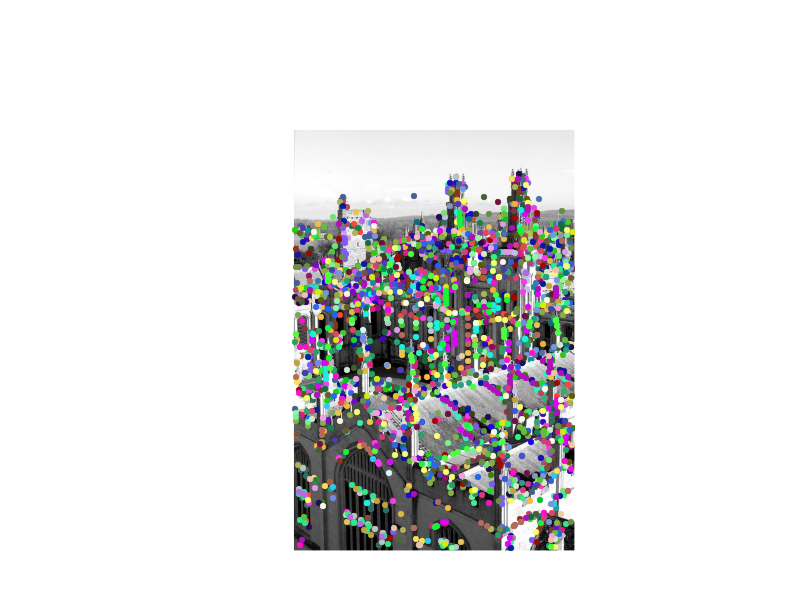
\includegraphics[width=\textwidth,height=.3\textheight,keepaspectratio]{randomimage1}
    \caption{\texttt{christ\_church\_000085.png}}
    \label{sfig:cc85}
  \end{subfigure}
  \begin{subfigure}{0.49\textwidth}
    \centering
    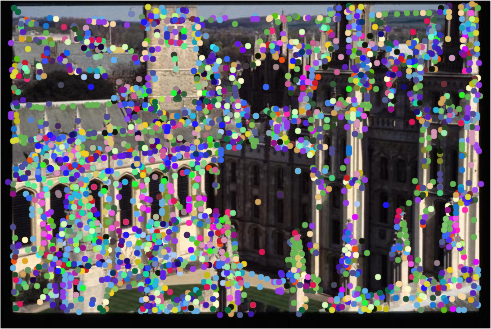
\includegraphics[width=\textwidth,height=.3\textheight,keepaspectratio]{randomimage2}
    \caption{\texttt{all\_souls\_000001png}}
    \label{sfig:as1}
  \end{subfigure}
  \begin{subfigure}{0.49\textwidth}
    \centering
    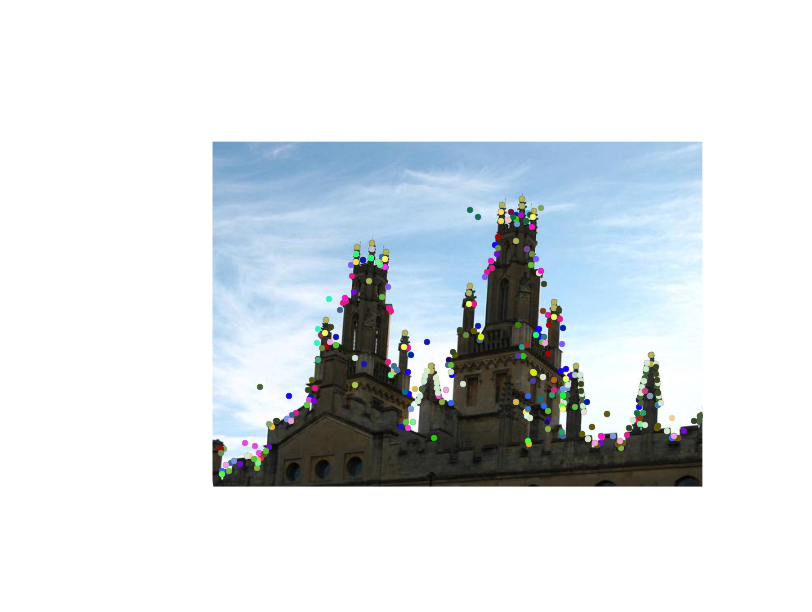
\includegraphics[width=\textwidth,height=.3\textheight,keepaspectratio]{randomimage3}
    \caption{\texttt{all\_souls\_000015png}}
    \label{sfig:as15}
  \end{subfigure}
  \begin{subfigure}{0.49\textwidth}
    \centering
    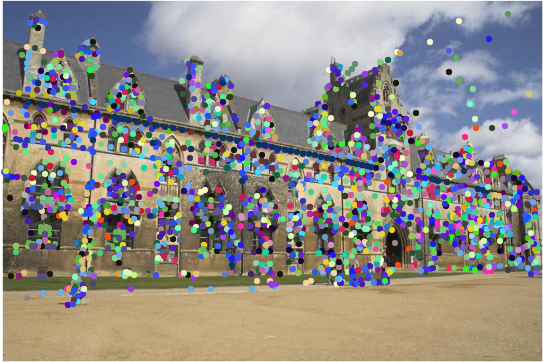
\includegraphics[width=\textwidth,height=.3\textheight,keepaspectratio]{randomimage4}
    \caption{\texttt{christ\_church\_000275png}}
    \label{sfig:cc275}
  \end{subfigure}
  \begin{subfigure}{0.49\textwidth}
    \centering
    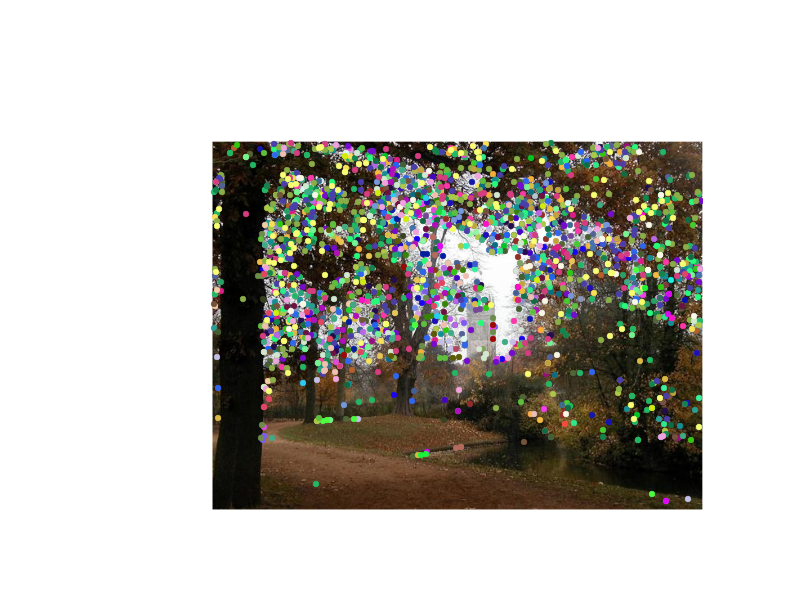
\includegraphics[width=\textwidth,height=.3\textheight,keepaspectratio]{randomimage5}
    \caption{\texttt{radcliffe\_camera\_000437png}}
    \label{sfig:rc437}
  \end{subfigure}
  \begin{subfigure}{0.49\textwidth}
    \centering
    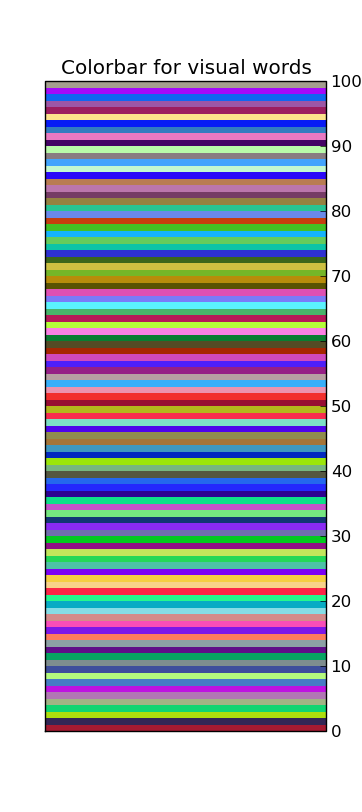
\includegraphics[width=\textwidth,height=.3\textheight,keepaspectratio]{colorbar}
    \caption{Legend.}
    \label{sfig:colorbar}
  \end{subfigure}
  \caption{SIFT vectors that have been assigned to words, plotted on images.  Figure~\ref{sfig:colorbar} functions as a legend for each feature: dots of the same color represent the same SIFT vector.  Its number can be looked up on this bar.}
  \label{fig:wordsonimage}
\end{figure}

The patches of five randomly selected words are shown in Figure~\ref{fig:words}.  The patches do look like each other, when you ignore the differences in hue (but not in intensity), rotation and scale.

\begin{figure}
  \begin{subfigure}{0.49\textwidth}
    \centering
    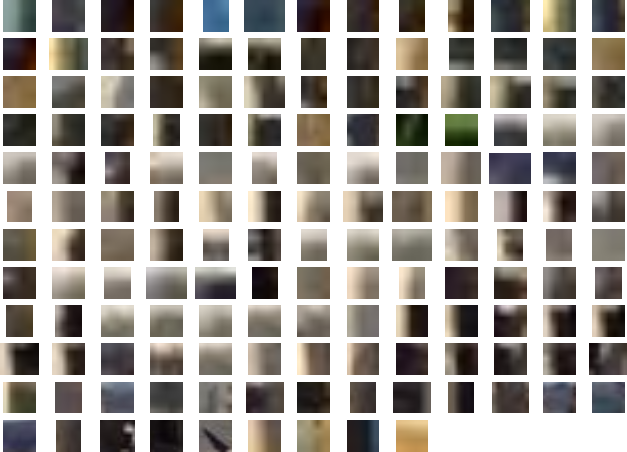
\includegraphics[width=\textwidth,height=.3\textheight,keepaspectratio]{word1}
    \caption{Word 69}
  \end{subfigure}
  \begin{subfigure}{0.49\textwidth}
    \centering
    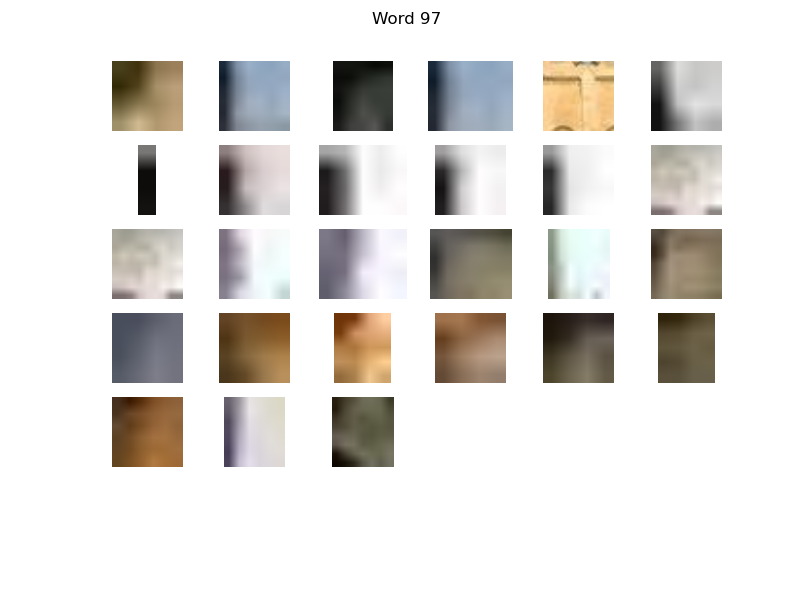
\includegraphics[width=\textwidth,height=.3\textheight,keepaspectratio]{word2}
    \caption{Word 65}
  \end{subfigure}
  \begin{subfigure}{0.49\textwidth}
    \centering
    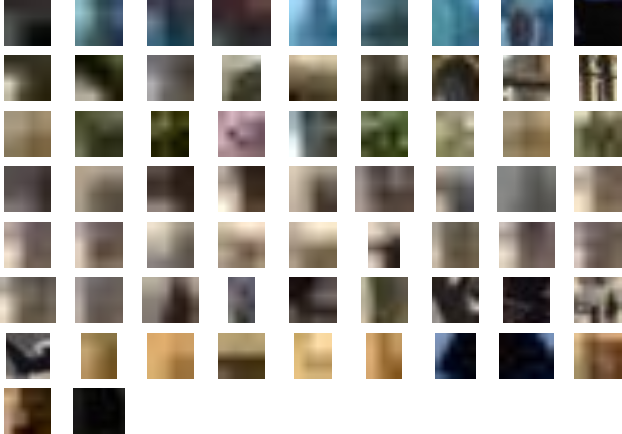
\includegraphics[width=\textwidth,height=.3\textheight,keepaspectratio]{word3}
    \caption{Word 10}
  \end{subfigure}
  \begin{subfigure}{0.49\textwidth}
    \centering
    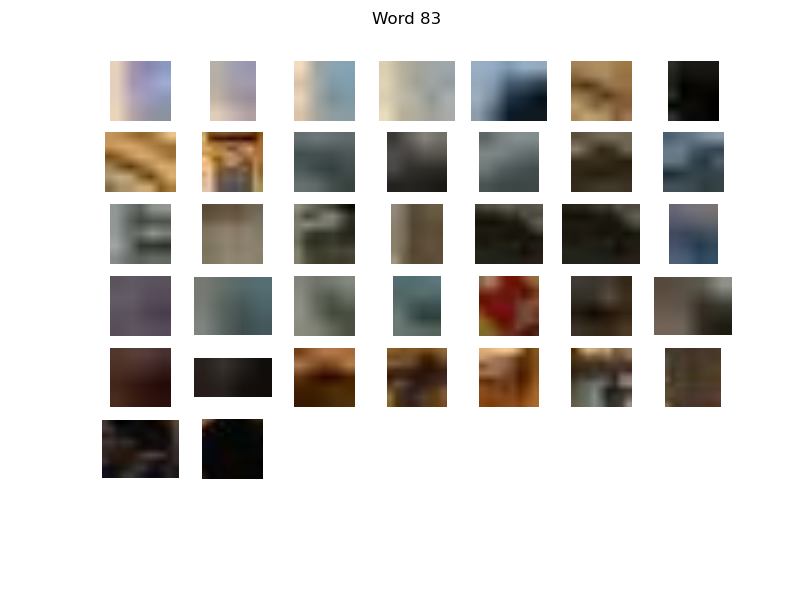
\includegraphics[width=\textwidth,height=.3\textheight,keepaspectratio]{word4}
    \caption{Word 2}
  \end{subfigure}
  \begin{subfigure}{0.49\textwidth}
    \centering
    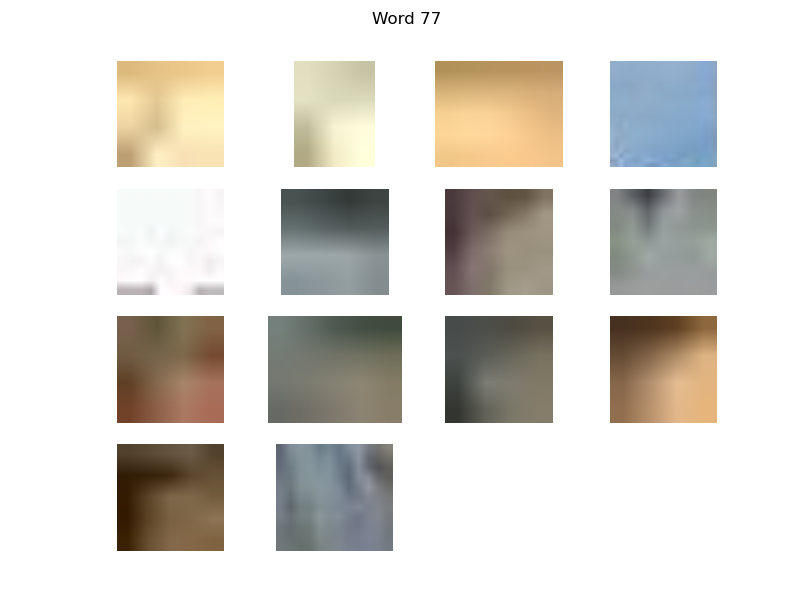
\includegraphics[width=\textwidth,height=.3\textheight,keepaspectratio]{word5}
    \caption{Word 38}
  \end{subfigure}
  \caption{Patches for five randomly selected words, as they occur in the images of Figure~\ref{fig:wordsonimage}.}
  \label{fig:words}
\end{figure}

Finally, the bag-of-words-histogram representation of the images of Figure~\ref{fig:wordsonimage} is presented in Figure~\ref{fig:histograms}.

\begin{figure}
  \begin{subfigure}{0.49\textwidth}
    \centering
    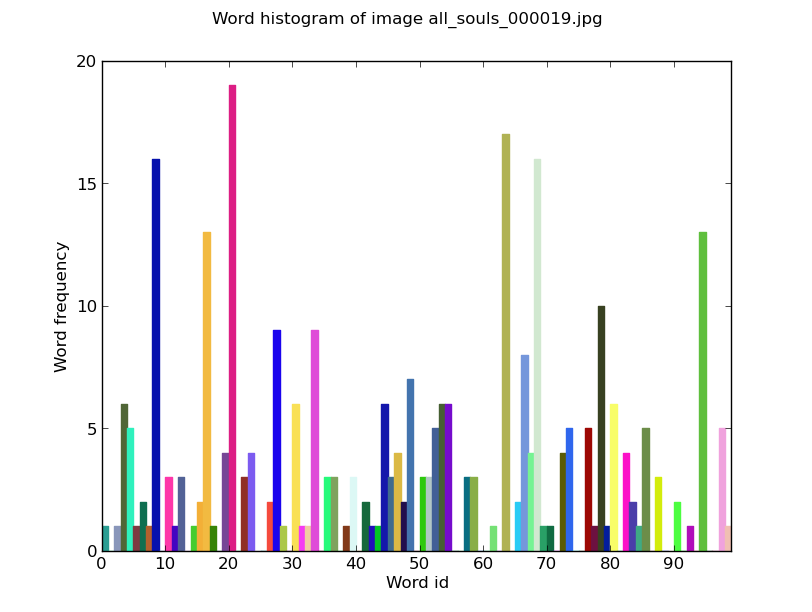
\includegraphics[width=\textwidth,height=.3\textheight,keepaspectratio]{histogram1}
    \caption{\texttt{christ\_church\_000085.png}}
  \end{subfigure}
  \begin{subfigure}{0.49\textwidth}
    \centering
    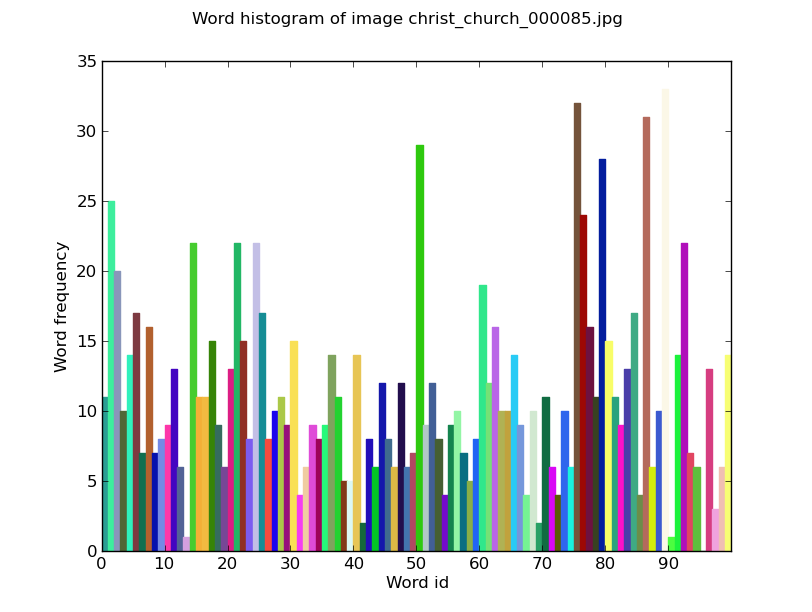
\includegraphics[width=\textwidth,height=.3\textheight,keepaspectratio]{histogram2}
    \caption{\texttt{all\_souls\_000001png}}
  \end{subfigure}
  \begin{subfigure}{0.49\textwidth}
    \centering
    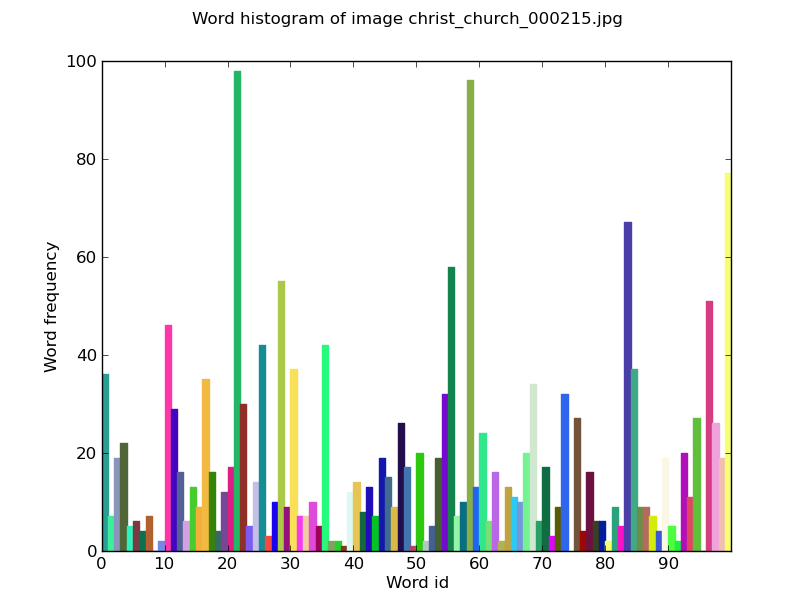
\includegraphics[width=\textwidth,height=.3\textheight,keepaspectratio]{histogram3}
    \caption{\texttt{all\_souls\_000015png}}
  \end{subfigure}
  \begin{subfigure}{0.49\textwidth}
    \centering
    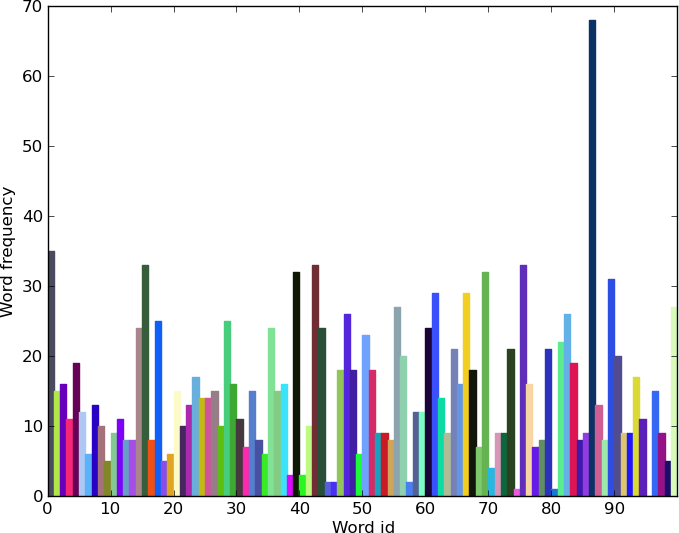
\includegraphics[width=\textwidth,height=.3\textheight,keepaspectratio]{histogram4}
    \caption{\texttt{christ\_church\_000275png}}
  \end{subfigure}
  \begin{subfigure}{0.49\textwidth}
    \centering
    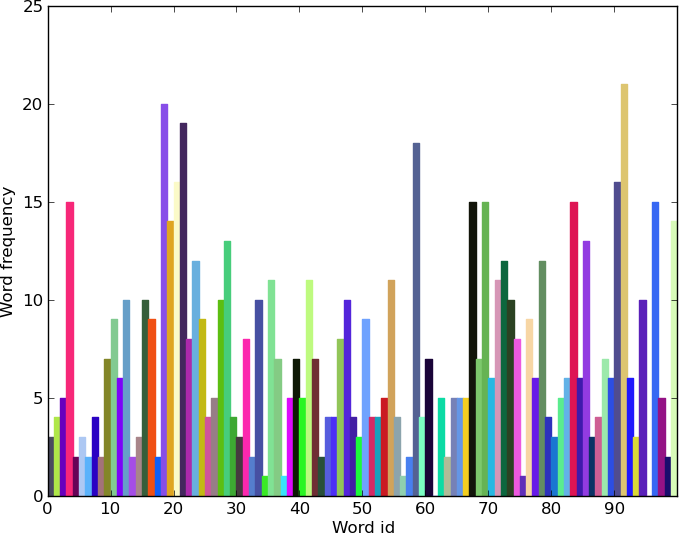
\includegraphics[width=\textwidth,height=.3\textheight,keepaspectratio]{histogram5}
    \caption{\texttt{radcliffe\_camera\_000437png}}
  \end{subfigure}
  \caption{Frequencies of visual words per image.  Each bar is visualised in the corresponding SIFT vector color.  Figure~\ref{sfig:colorbar} shows these colors.}
  \label{fig:histograms}
\end{figure}

\section{Visualizing Bag-of-Words retrieval}
\todo{see section 6}

\section{Evaluating Bag-of-Words histograms}
\todo{see section 5.2}

\section{Bonus 1}

\section{Bonus 2}

\end{document}
